\chapter{Layout Suche} \label{sec:LiteraturRecherche}
Das Ziel dieses Abschnitts ist es 2D-Layouts zu finden, die geeignet sind, um extrudiert zu werden und Software-Qualitätsmetriken in Form der in Abschnit \ref{sec:Problemstellung} definierten Form in 2.5D zu visualisieren. Alternativ können auch direkt 2.5D Visualisierungen gefunden werden, die geeignet sind, um Software-Qualitätsmetriken wie in der definitern Form zu visualisieren. 
In diesem Abschnitt stellen wir zunächst die Methodik vor, die wir bei der Recherche verwendet haben. Anschließend stellen wir die Ergebnisse der Recherche vor. 

\section{Methodik} \label{sec:Methodik}
Die hier verwendete Methodik orientiert sich an der Methodik der systematischen Literaturrecherche, wie sie in \textit{Procedures for performing systematic reviews}\cite{kitchenham2004procedures} beschrieben wird, ist aber leicht angepasst, da es vorallem um das finden und einordnen von Layouts geht und nicht direkt um das Bewerten und vergleichen von verschiedenen Arbeiten.

\subsection*{1. Forschungsfrage} \label{sec:Forschungsfrage}
Die Problemstellung dieser Arbeit an der hier gearbeitet wird ist bereits definiert:
\begin{quote}
    Lassen sich durch Analyse verwandter Arbeiten und bestehender Tools (zum Treemap Layout) alternative Layouts identifizieren, die eine bessere Grundlage für die Visualisierung von Code-Qualitätsmetriken bieten? (siehe Abschnitt \ref{sec:Problemstellung})
\end{quote}

Die Konkrete Forschungsfrage bzw. das Ziel dieser Rechere leitet sich aus dieser Problemstellung ab:
Unsere Recherche hat das Ziel, Layouts zu finden, die geeignet sind, um Software-Qualitätsmetriken in 2.5D zu visualisieren. Wir wollen dabei nicht nur spezifisch nach 2.5D visualierungen suchen, sondern auch nach 2D-Layouts, die geeignet sind, um in 2.5D extrudiert zu werden.

\subsection*{2. Suchstrategie} \label{sec:Suchstrategie}
Wir wollen sowohl wissenschaftliche Arbeiten als auch bestehende Tools und Ansätze finden, die sich mit der Visualisierung von Software-Qualitätsmetriken beschäftigen und analysieren, ob diese Ansätze geeignet sind, um auf unser spezifische Problemstellung übertragen zu werden.

Für die Suche nutzen wir zunächst Google Scholar wir wollen folgende Suche nutzen:

Wir wollen paper suchen, die sich mit der Visualisierung von Software-Qualitätsmetriken beschäftigen.
Wir teilen unsere Suche in zwei Teile auf:
Der fordere Teil beziet sich auf die Visualierung.
Und 
Der Hintere teil soll sicher gehen, dass es sich um Software-Qualitätsmetriken handelt, dafür muss auf jeden fall das wort software vorkommen und dann entweder "quality" oder "metrics". 
Beides muss im Paper vorkommen, um in unserer suche aufzutauchen.
Daraus ergibt sich folgende Suchanfrage:
("3D" OR "2.5D" OR "visualization" OR "treemap" OR "hierarchical data") AND ("software" AND ("quality" OR "metrics"))

Zur suche nutzen wir die erweiterte Suche von Google Scholar, um möglichst viele relevante Ergebnisse von verschiedenen Journalen und Anbietern zu finden.
Das Problem bei der erweiterten suche von Google scholar ist, dass sie sehr limitert ist und keine verschachtelten Suchanfragen unterstützt \cite{scholar_queries_2023}.
Deshalb teilen wir die Suche in zwei Teile auf: 
"3D" OR "2.5D" OR "visualization" OR "quality" OR "metrics AND "software"
und 
"treemap" OR "hierarchical data" OR "quality" OR "metrics AND "software"

Um trotzdem die gewünsche Suchanfrage nutzen zu können, um potentiell noch spezifischere und relevantere Ergebnisse zu erhalten, nutzen wir zusätzlich die \textit{Command Search} von IEEE Xplore, die auch verschachtelte boolsche Suchanfragen unterstützt \cite{ieee_xplore_boolean_2025}.

Wir schauen uns jeweils die ersten 20 Ergenisse an, da dies ein guter Kompromiss zwischen Relevanz und Anzahl der Ergebnisse ist.

Wir suchen nicht nur im Titel, sondern auch im Text, da es nicht immer alles expliziet im Title steht. 
Als Ziel des Papers, das ist zb. wichtig für die wörter quality oder metrics. Auch wenn viele das nicht explizit im Titel oder im abstract haben, wird trotzdem gibt es Paper diese daten als grundlage für die visualisierung verwendet, ohne dies wirklich explizit zu unterscheiden zwischen qualität und software selbst. ZB: Visualization of the Static Aspects of Software: A Survey

Außerdem suchen mit der normalen Google Suche nach existierenden Tools oder anderen Seiten, Ideen die genutzt werden können, um Software-Qualitätsmetriken zu visualisieren. Nutzen wir verschiedenste suchanfragen.

\subsection*{3. Inklusion und Exklusion Kriterien/Paper auswahl} \label{sec:InklusionExklusionKriterien}
Auf die Suchergebnisse wenden wir noch folgende Filter an, um unrelevante oder nicht zugängliche Ergebnisse zu exkludieren:

1. Wie bereits gesagt für google scholar: software ist ein muss, der rest ist optional in google scholar, auch wenn wir eigentlich gerne hätten, dass zumindest eines der wörter "quality" oder "metrics" vorkommt, um sicher zu gehen, dass es sich um Software-Qualitätsmetriken handelt und nicht um software-Visualisierung im allgemeinen (die wichtigkeit der unterscheidung wurde im Grundlagen Abschnitt \ref{sec:SoftwareVisualisierung} erleutert) deswegen filtern wir die suchergebnisse auch manuell, um sicher zu gehen, dass es sich um relevante Ergebnisse handelt: zB: Software Architecture Visualization: An Evaluation Framework and Its Application \cite{gallagher2008software}

2. in englisch oder deutsch - aber alles war sowieso auf englisch, aufgrund der Suchbegriffe, außer ein spanisches paper: Software visualization tools and techniques: A systematic review of the literature\cite{cruz2016software}

3. Frei zugänglich über alle herkömmlichen anbieter: IEEE, sprignerlink, acm digital library, researchgate,... Das sind die meisten außer zb. Understanding software evolution using a combination of software visualization and software metrics \cite{lanza2002understanding}

4. Außerdem generell innhalblich auch passen. zb. Open source software for visualization and quality control of continuous hydrologic and water quality sensor data \cite{horsburgh2015open}

5. wird wirklich eine visualisierung vorgestellt? Wenn in dem paper entweder, mindestens eine 2D layout vorgestellt wird oder wenn mindestens eine 2.5D Visualisierung vorgestellt wird. zb.: Existing model metrics and relations to model quality \cite{mohagheghi2009existing}

Für die normale Google suche, verwenden wir verschiedenste heuristische Filter um werbung, Dienstleistungsanbieter und andere irrelevante Ergebnisse zu filtern.

\subsection*{4. auswertung der paper und extraktion der layouts} \label{sec:AuswertungPaper}
Filtern der Layouts, könnten diese für 2.5D geeignet sein?
Sammeln und gruppieren der geeigneten verschiedener Layouts
Entscheiden für layouts



Wie entscheide ich, ob ein layout geeignet ist:
- Es sollte eine Art von Metrik oder Wert darstellen können.
- Es sollte eine Art von Layout haben, dass die Struktur der Hierarchie darstellt.
- Es sollte ins drei dimensionale extrahierbar sein.
- Es soll auch ohne spezielle Einfärbung im 2D funktionieren - eventuell nur die ordner einfärben

\subsection*{5. qualitäts analyse: (Analyse der Layouts und entscheidung welche layouts in dieser arbeit behandelt werden)} \label{sec:QualitaetsAnalyse}

\section{Durchführung der Suche}
Hier stellen wir zunächst die Ergebnisse der Suche vor nachdem bereits die Filter angewendet wurden.

Erste Google Scholar Suche:
1. Voronoi treemaps for the visualization of software metrics \cite{voronoiTree}
- Voronoi Treemap Layout
- sie sagen dass problem ist dass geschwister nicht einfach von anderen benachbarten knoten unterschieden werden können, wir versuchen dass mit den margins zu lösen
- als erste probieren sie nicht rechtecke sondern polygone
\begin{quote}
    The problem is provoked by the square-like shape of the rectangles, and because the edges are only horizontally and vertically aligned, whereby the edges of the different objects appear to run into each other. [...] A solution for this problem is the layout of Treemaps based on non-rectangular objects.\cite[3]{voronoiTree}
\end{quote}
\begin{quote}
    these polygons are clearly distinguishable because of their irregular shapes, and their aspect ratio converges to one \cite[6]{voronoiTree}
\end{quote}
Aber selbst sie fügen kanten hinzu - und größere he höher
außerdem nutzen sie Sättigung um noch mehr die Tiefe und die Hierarchie darzustellen
- Kritik: sie wollen treemap geschwisterproblem lösen, schaffen dies aber durch ihren ansatz nicht wirklich und fügen dann doch wieder kanten und farbe hinzu um das zu unterstützen

2. Visualization-based analysis of quality for large-scale software systems \cite{visbasedlarge}
- Zeichnen auch Quader. diese Quader haben immer die selbe grundfläche
- metriken werden dargestellt durch 1. die höhe des Quaders, 2. die farbe des Quaders, 3. die rotation (zwischen 0 und 90 Grad) 
- deren problem ist also nur die platzierung der Quader
- KRitik: gefällt mir nicht so gut, vorallem die Roation, außerdem viel platz verschwendet. Sie sagen, dass gedreht schlecht ist. aber 90 Grad sieht nicht so schlimm aus wie 45 grad. dumm
-Struktur auf klassen und paket ebene -> das macht es natürlich einfacher, da es generell wenier packete als ordner gibt (packete können auch nochmal in ordner unterteilt sein)
- Am ende nutzen sie für die platzierung treemap und Sunburst
- Da die fläche fix und diskret ist, erweitern sie sowohl den treemap als auch den sunburst algorithmus
- Treemap: beim slicen, wenn der platz zu schmal wird, wird der platz einfach erweitert, für alle knoten, in eine richtung -> sehr viel leerer platz, auch wenn sie versuchen das so gering wie möglich zu halten
\enquote{burst can still result in the insertion of holes in the representations. In simple illustrations such as in Figure 4, this looks like a serious problem. However, our framework is designed to study systems made of hundreds and thousands of elements. In fact, in the average cases (real softwares) that we tested, it did not prove a problem at all in our visualization.}
Zeigt, wie wichtig unsere datenanalyse ist, da es wichtig ist die visualisierung für reale daten zu machen und nicht nur simple beispiele

\begin{figure}
    \centering
    \includegraphics[width=0.8\textwidth]{images/literatur/visbasedlarge.png}
    \caption{(Oben) Modifizierte Treemap-Technik und (unten) modifizierte Sunburst-Technik. Beide repräsentieren PCGEN, ein Tool zur Charaktererstellung in RPG (1129 Klassen). \cite[5]{visbasedlarge}.}
    \label{fig:visbasedlarge}
\end{figure}
vielleicht etwas zu simple gedacht??


\enquote{there is still room for improvements, mainly to better exploit the entire display space}\cite[8]{visbasedlarge}

3. Visualization of the static aspects of software: A survey \cite{staticSurvey}
In diesem Paper werden verschiedene Visualisierungen vorgestellt. dieses paper auch schon in verwandten arbeiten erwähnt.
Es werden 6 verschiedene Visualisierungen vorgestellt, die auch auf unseren usecase passen. 

Sehr gute arbeit, da sie einige visualiasierungen vorstellen.
2D: Treemap, Sunburst, Circle Packing, voronoi

Verschiedene Stadtmethaphern
Eine stadt und insel methapher,
solar system methapher, welche gleich auch noch genauer beschrieben wird
hierarchical net

Zeigen auch, dass das was am meisten verwendet ist stadt methapher und generell treemaps

Ansonsten auch viele andere visualisierungen, die nicht so gut passen, weil es speziell um architektur, evolution oder verbindungen geht.


4. Visual realism for the visualization of software metrics \cite{visRealism}
Nutzen normale Cushion Treemaps und schattierung und struktur um metrik werte dar zu stellen
nutzen aber auch package struktur, die deutlich einfacher ist als ordner struktur -> nur drei level

5. An overview of 3D software visualization \cite{overview3D}
Zeigen alles von 2D, 2.5D und 3D



6. CityVR: Gameful software visualization \cite{cityVR}
- Stellen stadt methapher in 3D vor
- fokus auf gamification
- layout ist ähnlich wie bei codecity

7. A solar system metaphor for 3D visualisation of object oriented software metrics \cite{solarSystem}
Schauen diese metriken an:
Lines of Code(LOC) NCSS
Number of Children(NOC) DF
Weighted Methods (WMC) NCSS
Coupling Between Objects(CBO) DF
Depth of Inheritance Tree (DIT) DF
ganz neue methapher: solar system

\begin{figure}
    \centering
    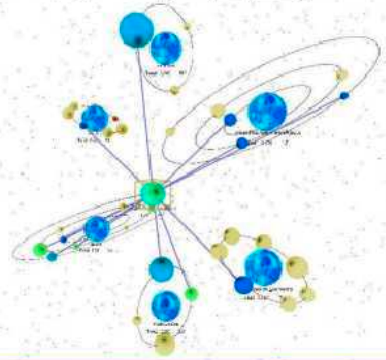
\includegraphics[width=0.6\textwidth]{images/literatur/solarSystemMethaphor.png}
    \caption{Solar System Metapher für 3D Visualisierung von objektorientierten Softwaremetriken. Die farben des bildes sind invertiert, um die lesbarkeit im ausdruck zu verbessern. \cite[4]{solarSystem}}
\end{figure}
Man erkennt, dass es wirklich 3D ist und nicht 2.5D
Sie kritisieren, dass die Stadt-Metapher nicht so gut ist, da sie nicht wirklich 3D ist. Und keine Komplexen Zusammenhänge dargestellt werden können. Überdeckung.

Sonnen sind pakete. Planeten sind Klassen, wobei die farbe den typ der klasse angibt. 
Umlaufbahnen stellen die Vererbungsebenen innerhalb des Pakets dar. Planeten in derselben Umlaufbahn gehören zur gleichen Vererbungshierarchie
Die Größe der Planeten ist eine Metrik (die anzahl der zeilen code)
Verbindungen zeigen kopplung zwischen Klassen an.

Es werden aber nur relativ kleine Pakete visualisiert, mit nur so ca. 30-40 klassen.

es können nur 2 metriken dargestellt werden, eine auf klassenebene, eine auf verbindungsebene.
Man könnte noch die Farbe als metrik nutzen und man könnte nicht auf klassen sondern auf file ebene betrachten (geht ja eigentlich immer)
Es wird gefühlt sehr viel leerer platz verschwendet
Es gibt doch auch einige überdeckungen, da die umlaufbahnen, teilweise hinter anderen planeten hergehen.
Man könnte das ganze als 2D Layout verwenden und dann kugelförmig extrudieren, das 
ich stelle es mir unvorteilhaft vor

8. EvoSpaces: 3D Visualization of Software Architecture. \cite{EvoSpaces}
Sie untersuchen verschiedene darstellungen 
simple darstellungen wie einfache quader oder auch wirkliche häuser
metriken werden transparenz, höhe, größe, textur,...
dabei können mehrere metriken verwendet werden
gebäude sind klassen oder dateien. verbindungen sind röhren bzw. strahle die oben aus einem gebäude herauskommen un dann im bogen in ein anderes gebäude von oben hineingehen

\begin{figure}
    \centering
    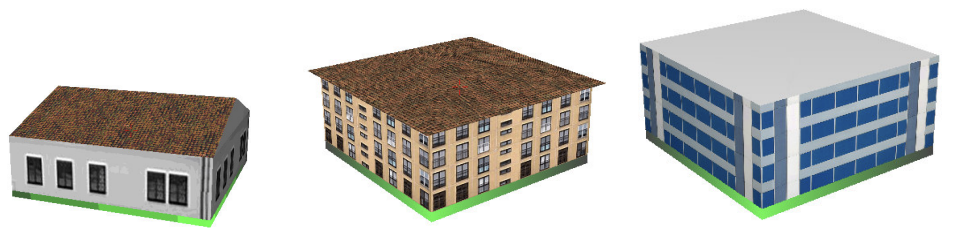
\includegraphics[width=0.8\textwidth]{images/literatur/evoSpaces.png}
    \caption{Ein Beispiel für eine EvoSpaces Visualisierung. Die Gebäude repräsentieren Klassen, je nach Metrik-WErt werden diese in unterschiedliche Kategorien eingeteilt (z.B. bis zu 50 LOC - Wohnhaus, 51-200 LOC - Apartmentblock,...) \cite[3]{EvoSpaces}.}
    \label{fig:evoSpaces}
\end{figure}

sie stellen aber nur zwei layouts vor, die nicht die struktur zeigen, sondern auch wieder eine Metrik darstellen. zb. im kreis und älteste datei am weitesten innen.

\begin{figure}
    \centering
    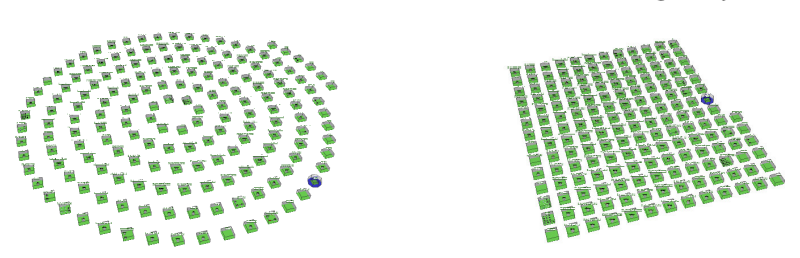
\includegraphics[width=0.8\textwidth]{images/literatur/evoSpaceLayout.png}
    \caption{Die zwei Layouts, die EvoSpaces verwendet. Links: Konzentrisch und Rechts Schachbrettartig. \cite[3]{EvoSpaces}.}
    \label{fig:evoSpaceLayout}
\end{figure}


9. 3D representations for software visualization \cite{3dsoftwareMarcus}
weiterentwicklung von 2d pixel bars ins 3D, weil mehr metriken und besser die verbindungen darstellbar
softvis3d
läuft auch auf basis von metriken auf datei ebene
sehr detailiert, viel kleineteiligere darstellung, da einzelene code zeilen dargestellt werden
vorallem für die entwicklung gedacht
überdeckung wollen sie mit transparenz lösen
layout angeordnet nach zeile für zeile
keine hierarchie


10. Software cartography: Thematic software visualization with consistent layout \cite{softwareCartography}
Es wird eine topographische Kartenmetapher verwendet
Dateien sind Hügel, die Höhe ist eine Metrik (zB. LOC)
Das layout wird mit hilfe eines speziellen Multidimensionale Skalierungsalgorithmus (Hit-MDS) erstellt
als stress wert der funktion wird die Lexikalische Distanz zwischen den Dateinamen verwendet (ist vielleicht gut wenn man schnell bestimmte dateien finden will, aber nicht so gut für die hierarchie und auch weit weg von der software selbst)
sie zeigen noch eine erweiterung mit icons auf den bergspriten, die auch noch eine metrik darstellen können
wurde besonders entwickelt mit dem Ziel von software evolution

ich sage, das ist eine interessante grundidee und anders

\begin{figure}
    \centering
    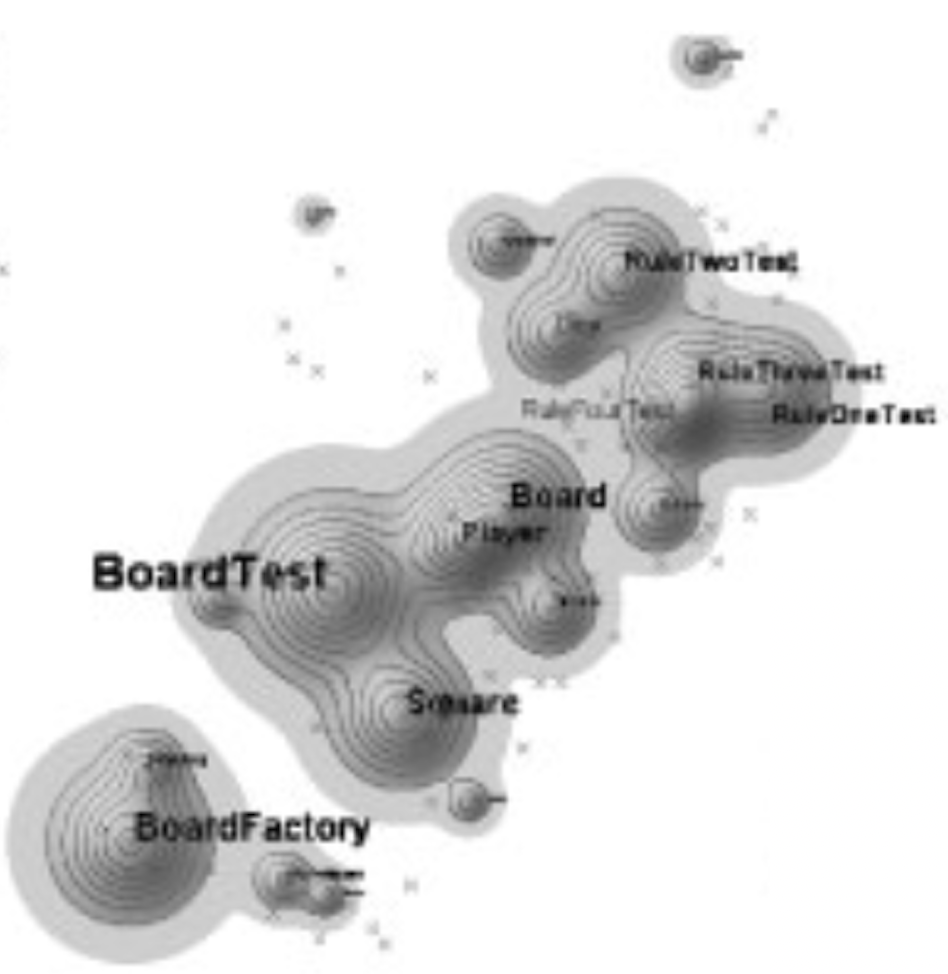
\includegraphics[width=0.8\textwidth]{images/literatur/softwareCartography.png}
    \caption{Software Cartography: Topographische Kartenmetapher für Software Visualisierung. Die Hügel repräsentieren Dateien, die Höhe ist eine Metrik (z.B. LOC). \cite{softwareCartography}.}
    \label{fig:softwareCartography}
\end{figure}

zweite Google scholar suche:
Doppelte Treffer: 4 zB.: Visualization-based analysis of quality for large-scale software systems \cite{visbasedlarge}
1. Exploring Relations within Software Systems Using Treemap Enhanced Hierarchical Graphs \cite{exploringRelations}
auf oberer Ebene wird energy model of Noack and Lewerentz genutzt um einen graphen zu malen. 
dieser graph kann auch mehrere hierarchie ebenen visualisieren, dabei wird farbe als unterstüzendes mittel genutzt, um die verschiedenen pakete oder order zu unterscheiden.
Jeder knoten hat dann nochmal intern eine Treemap, die die Struktur des knotens zeigt

\begin{figure}
    \centering
    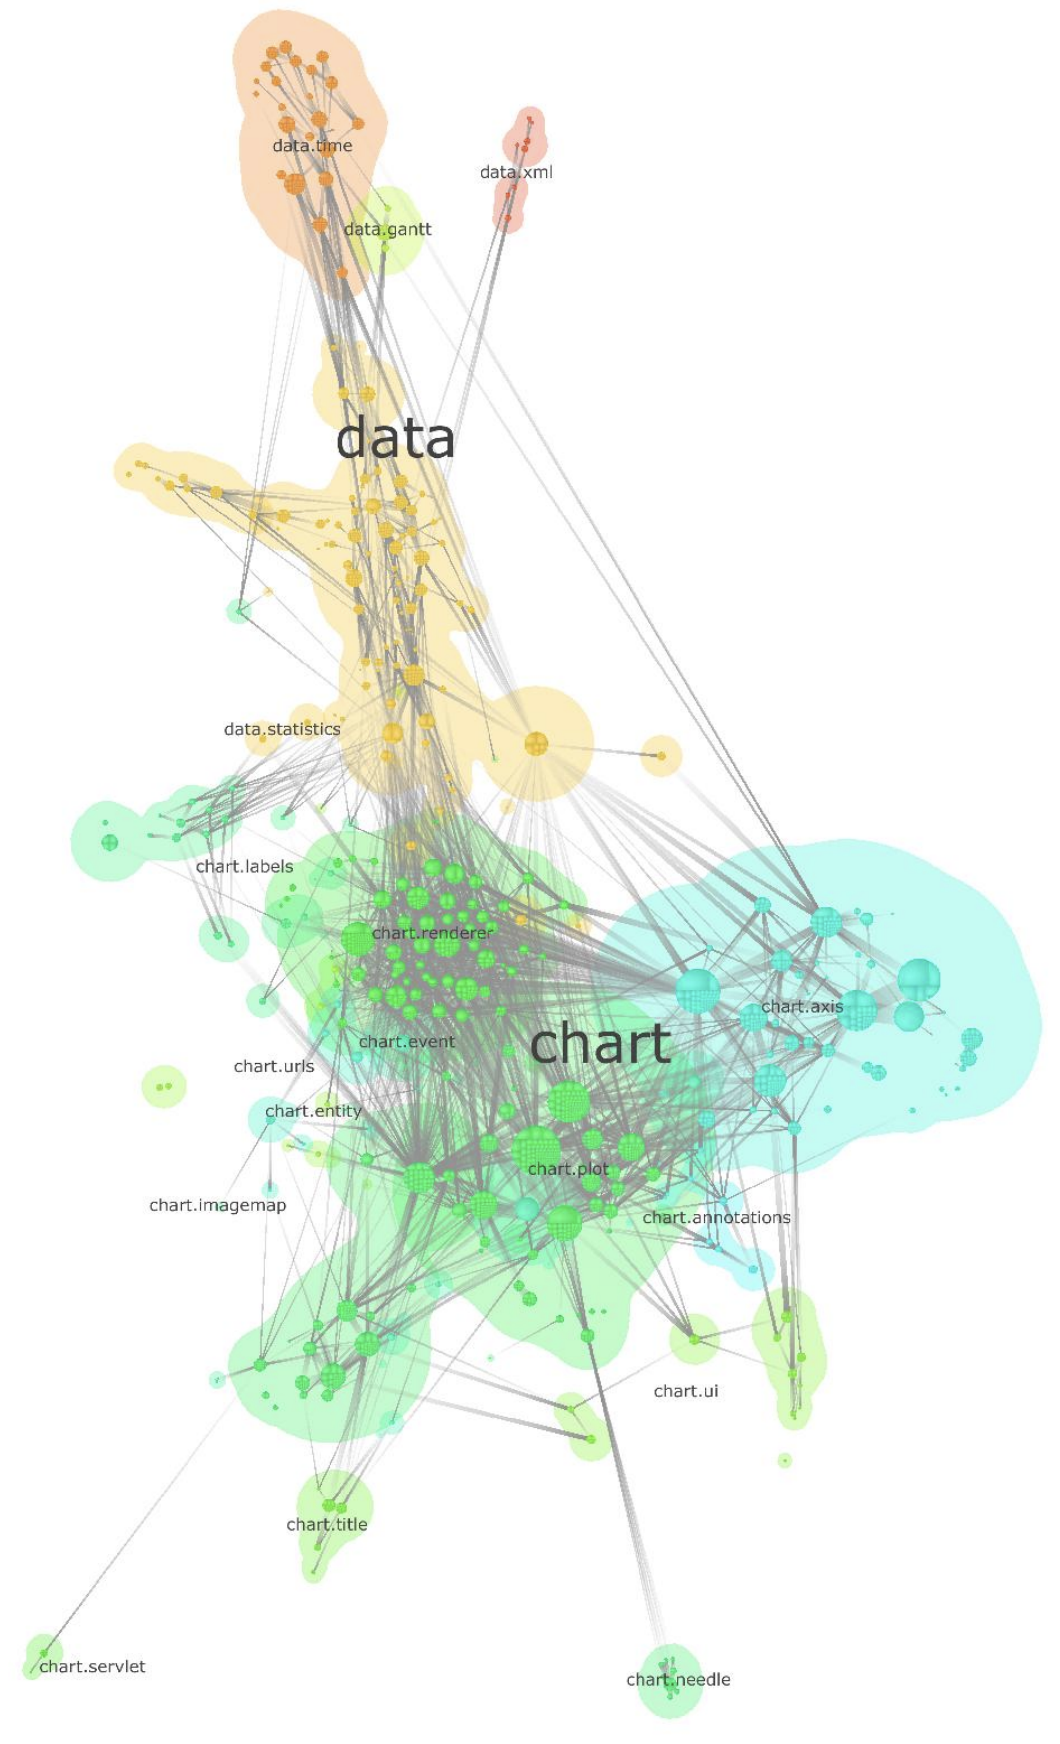
\includegraphics[width=0.8\textwidth]{images/literatur/expoloringRelations.png}
    \caption{Exploring Relations within Software Systems Using Treemap Enhanced Hierarchical Graphs. Die obere Ebene ist ein Graph, der die Beziehungen zwischen den Paketen zeigt. Die untere Ebene (in den einzelenen kreisen nur klein zu sehen) ist eine Treemap, die die Struktur des Pakets zeigt. \cite[5]{exploringRelations}.}
    \label{fig:exploringRelations}
\end{figure}

interaktion mit zoomen ist von nöten. 
Alles bisher noch in 2D

2. Visualizing Software Metrics in a Software System Hierarchy \cite{visSoftwareMetricsBook}
im grunde eine link treediagram, 
Metrik stripes - metrische streifen, zeigen über breite und farbe verschiedene metriken an

\begin{figure}
    \centering
    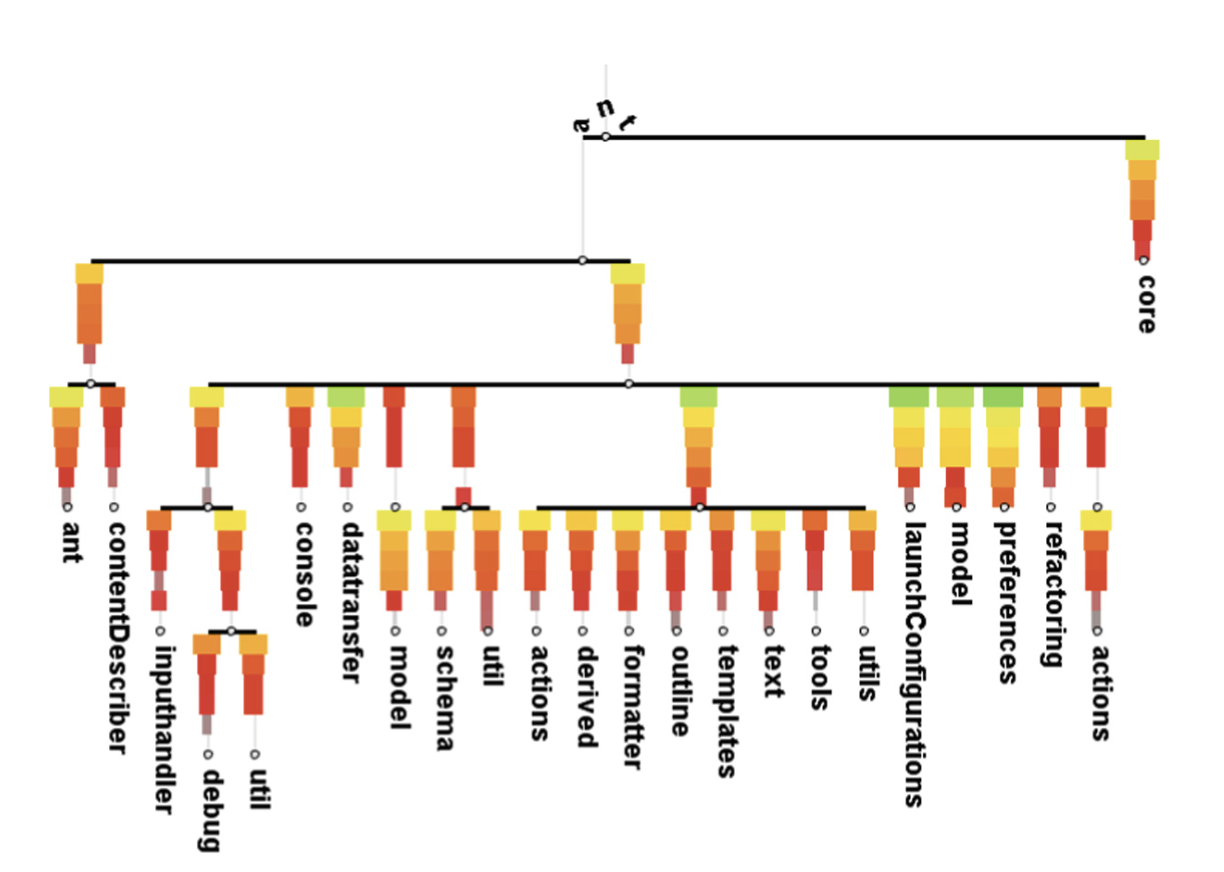
\includegraphics[width=0.8\textwidth]{images/literatur/vishierarchy.png}
    \caption{Im grunde ein link-treediagram, das mit \textit{Metric Stripes} verschiedene metriken darstellt. \cite[740]{visSoftwareMetricsBook}.}
    \label{fig:visHierarchy}
\end{figure}

layout wird wie in groundlagen gesagt, sehr schnell unübersichtlich.

3. A Stable Greedy Insertion Treemap Algorithm for Software Evolution Visualization \cite{stableGreedyInsertion}
stellen nur neuen treemap algorithmus vor, der fokus auf stabilität hat
diese wruden erstmals hier vorgestellt \cite{Goertler2017BubbleTreemapsUncertainty}

4. Visualizing Program Quality – A Topological Taxonomy of Features  \cite{visualizingProgramQuality}
eigentlich gar nicht für software qualität, aber schlagen die bubble treemap vor

\begin{figure}
    \centering
    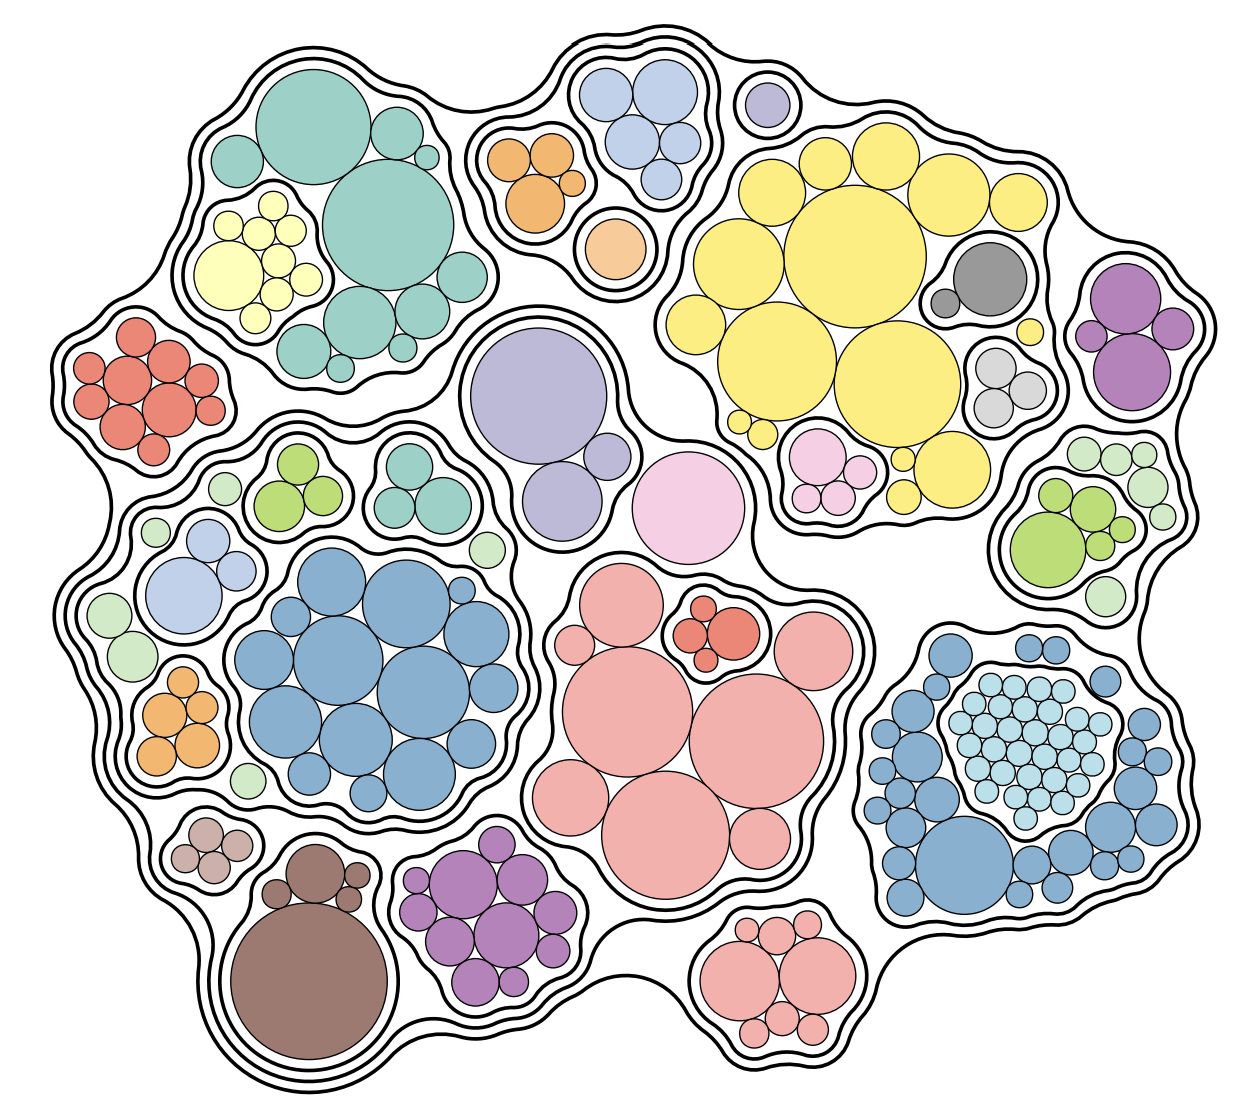
\includegraphics[width=0.8\textwidth]{images/literatur/bubbleTreemap.png}
    \caption{Beispiel für eine Bubble Treemap \cite[7]{Goertler2017BubbleTreemapsUncertainty}}
    \label{fig:bubbleTreemap}
\end{figure}

5. Stable and predictable Voronoi treemaps for software quality monitoring \cite{stablePredictableVoronoi}
erweitern voronoi
3 metriken: 1. farbe 2. größe 3. reihenfolge der anordnung/bzw positionierung
idee ist als 3. metrk den fully qualified name zu nutzen um so die topologie der hierarchie darzustellen
-> Ziel vergleich zwischen verschiedenen versionen


6. Visualization and evolution of software architectures \cite{visualizationEvolution}
%auch related work?

IEEE Suche:
Doppelt: 3 zB. Visualization of the Static Aspects of Software: A Survey \cite{staticSurvey}
1. Metrics-based 3D visualization of large object-oriented programs \cite{metricsBased3DVisualization}
auch größe und farbe als metrik

Einzelne Kugeln, Würfel,... im 3d raum, die mit linien verbunden sind, je nach verbindung
das layout ist nach einem gleichheitswert der klassen angeordnet, dieser wert kann alles sein, entweder metrik oder platz etc.

\begin{figure}
    \centering
    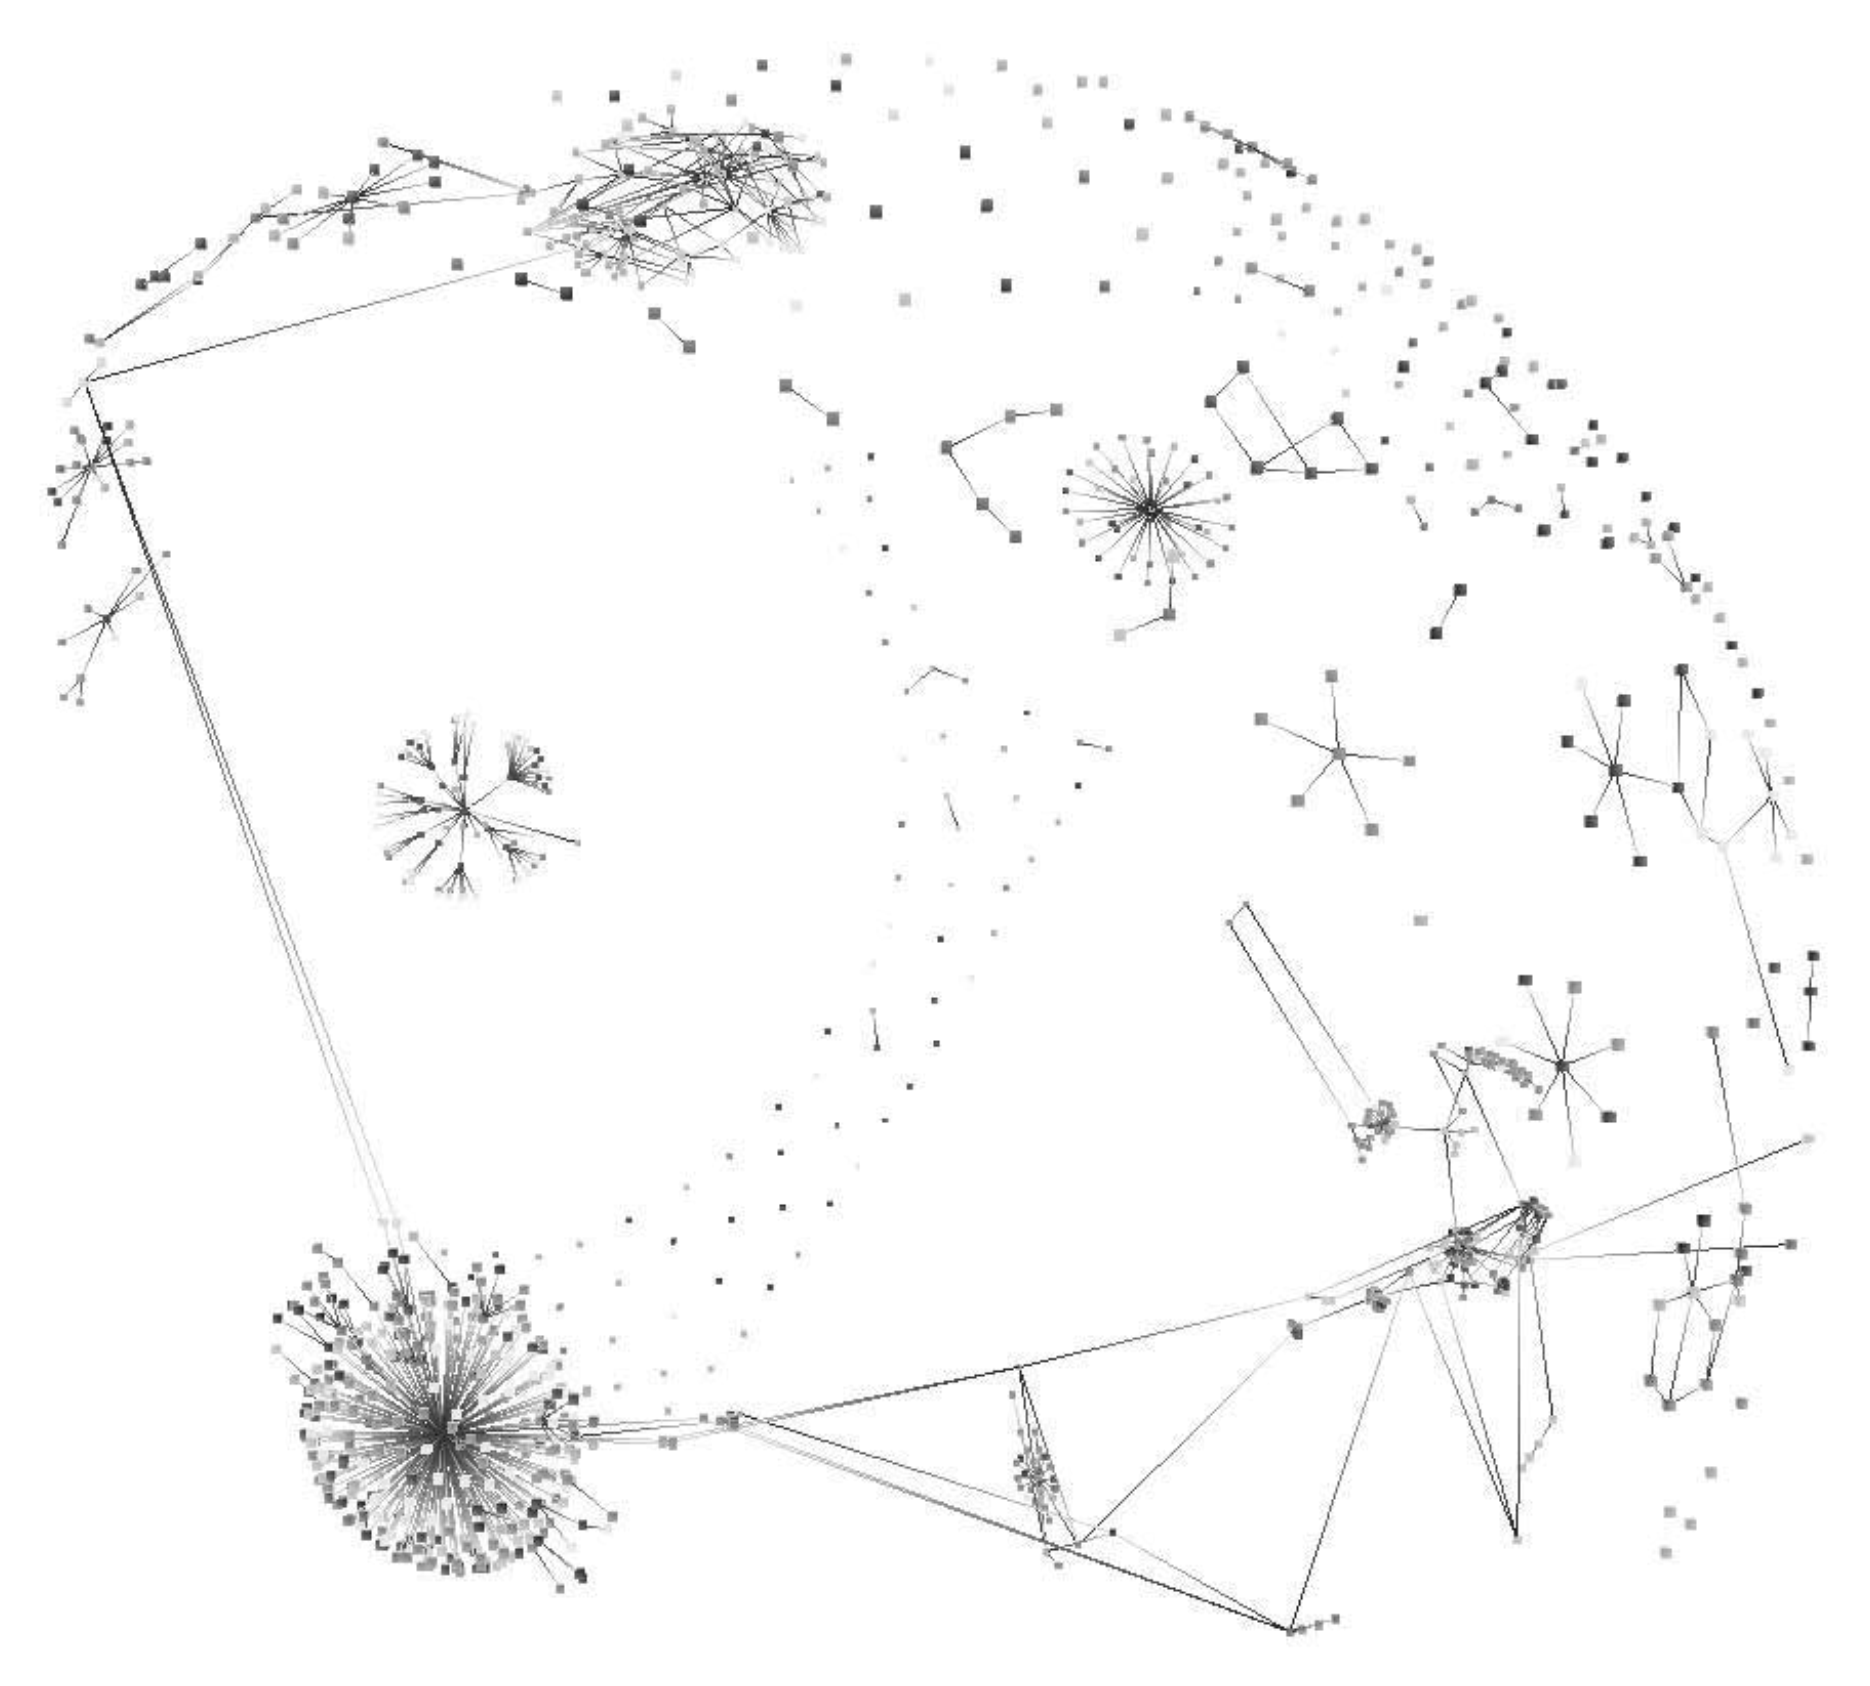
\includegraphics[width=0.8\textwidth]{images/literatur/metricsBased3DVisualization.png}
    \caption{Die vorgestellte visualierungen zeigt, wie klassen in 3D gemappt werden anahdn von similarity score  \cite[5]{metricsBased3DVisualization}.}
    \label{fig:metricsBased3DVisualization}
\end{figure}



2. Visualizing Metric Trends for Software Portfolio Quality Management \cite{visualizingMetricTrends}
Stellen einfach eine Plattform vor, die verschiedene Metriken über zeit visualisiert
mit linien plots und balken diagrammen für komplette software - nicht wirklich relevant für uns


3. E-Quality: A graph based object oriented software quality visualization tool \cite{eQuality}

\begin{quote}
    First, we examine a small-sized project to be able to easily illustrate the features of E-Quality. \cite[5]{eQuality}
\end{quote}
nur vergleich mit folder based navigations methode

\begin{figure}
    \centering
    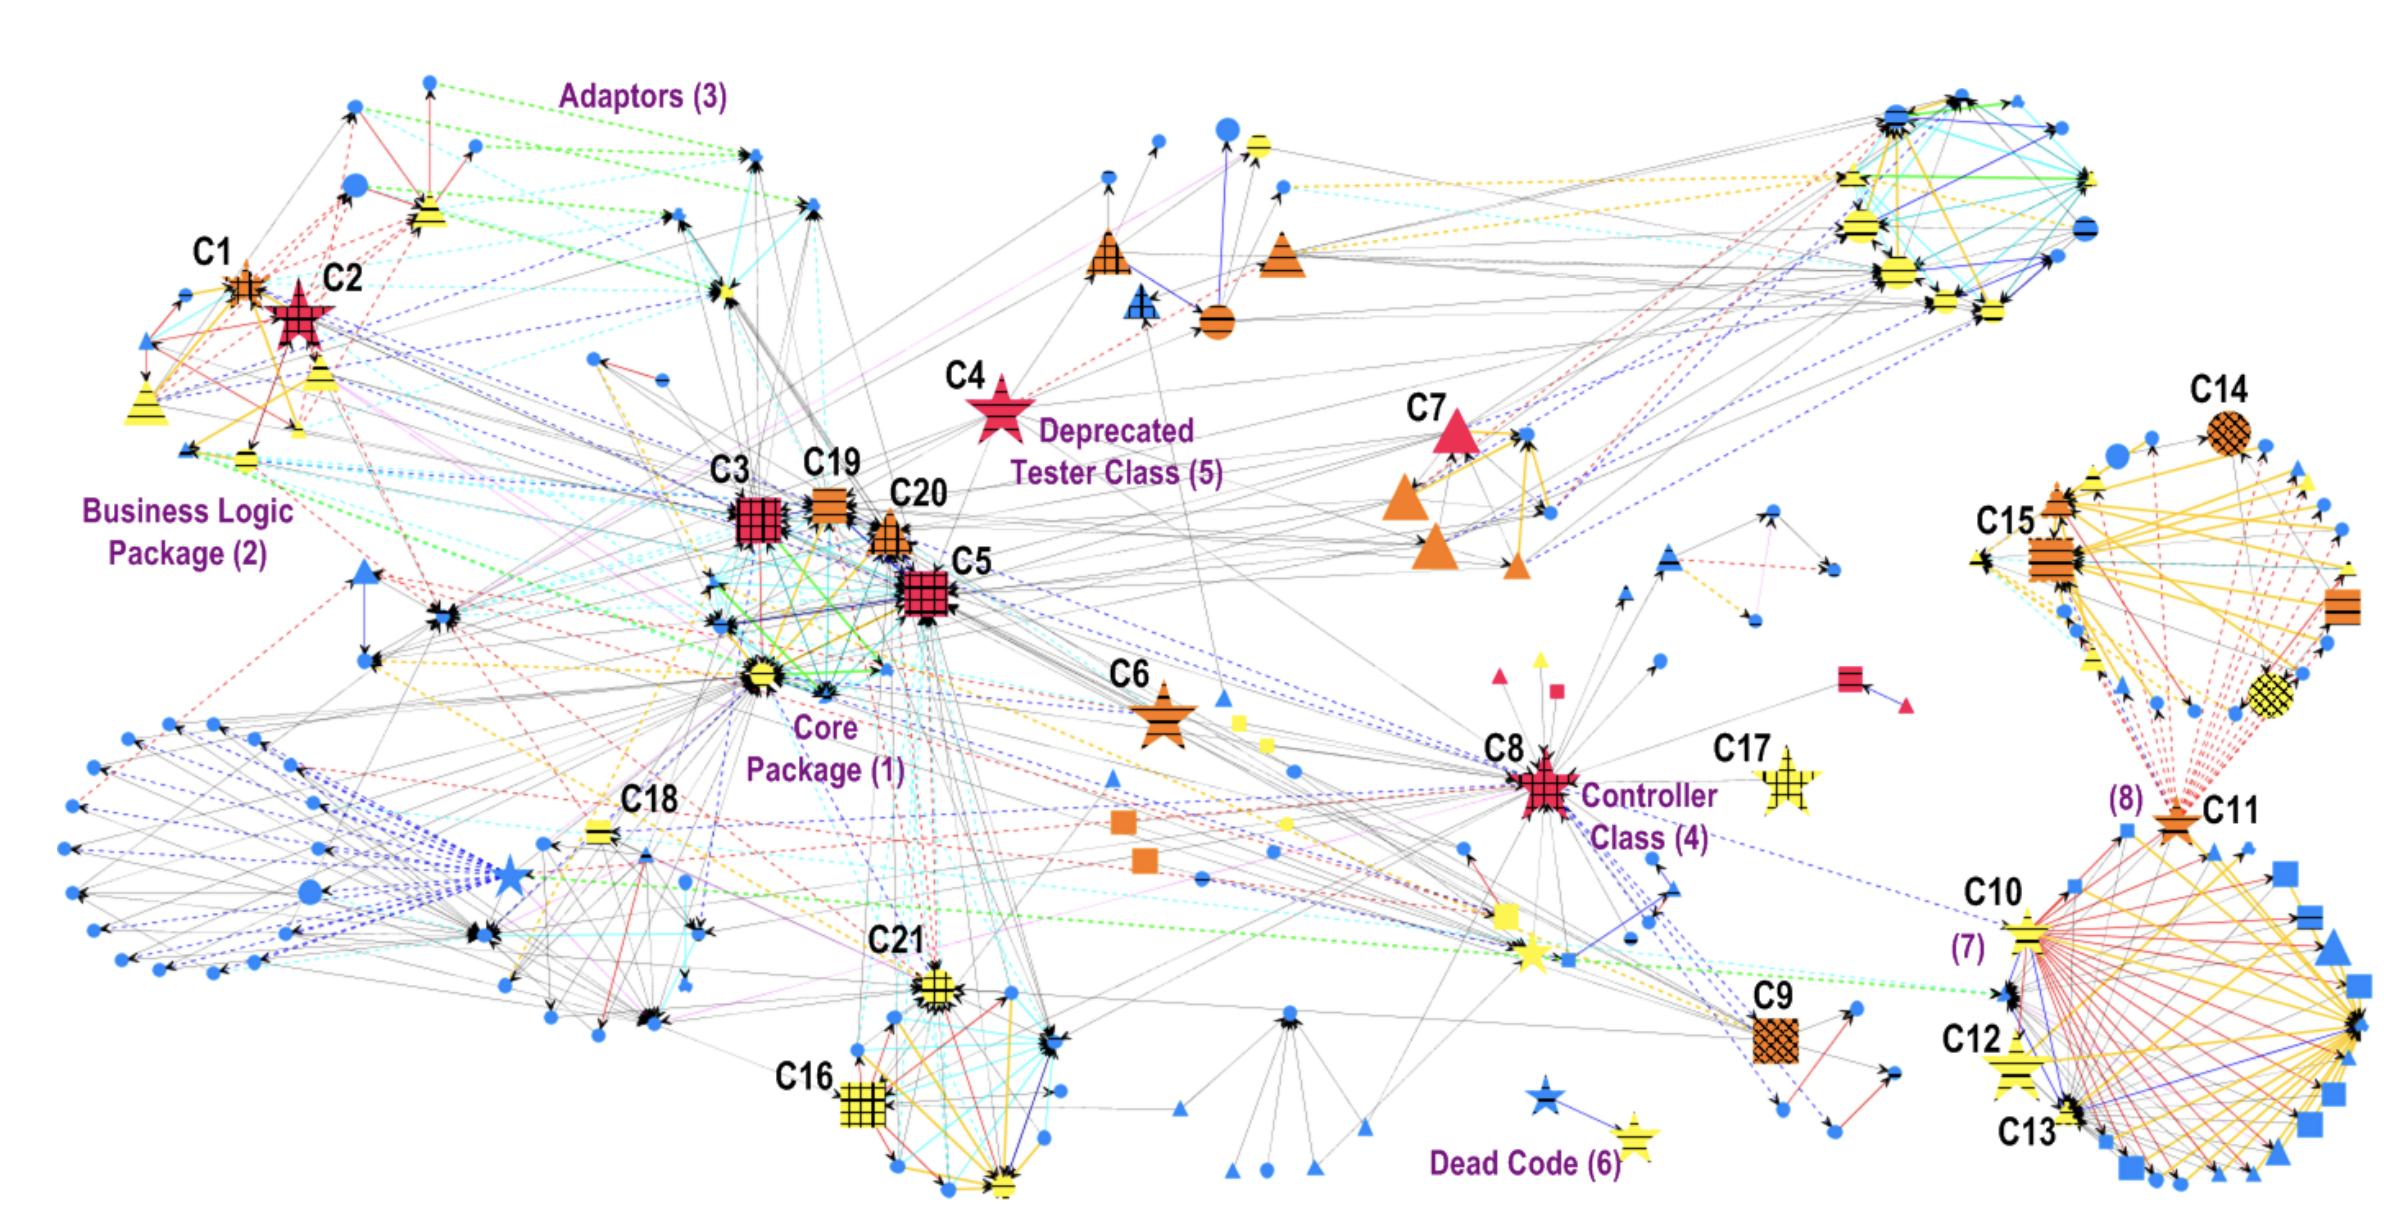
\includegraphics[width=0.8\textwidth]{images/literatur/equality.png}
    \caption{E-Quality: Ein graph basiertes objektorientiertes Software-Qualitätsvisualisierungstool. \cite[5]{eQuality}.}
    \label{fig:eQuality}
\end{figure}

packete werden kreisförmig angeordnet
Metriken haben auswirkung auf, muster, größe, farbe, form


4. Visualization of Software Quality Expert Assessment \cite{visSoftQualExpert}
auf projekt ebene



5. QScored: An Open Platform for Code Quality Ranking and Visualization \cite{QScored}
stellen eigentlich nur plattform vor
visualisieren mit treemaps und sunburst und dependecy graph


6. Using the City Metaphor for Visualizing Test-Related Metrics \cite{citMetaphorTestMetrics}
Stadt methapher in minecraft
Gebäude sind sehr detailiert und bilden methoden, attribute, metriken, interfaces, ... alles mögliche ab
eher eine spielerei, aber im grunde layout wie code city

7. Visual Analytics of Software Structure and Metrics \cite{visAnaSoftStructure}
Nutzen den city view: von ecity \cite{ecity}
eCITY: A Tool to Track Software Structural Changes Using an Evolving City





Google Tool suche:
Gefilter werden paper, wenn sie kommen. Nur webseiten werden geöffnet
Software Quality Visualizer


Software Metric Visualizer/software quality analysis/ software visualisation tool/ 
dabei auch die filter: 1. software quality vis 2. existing tool 3. keine paper, 
viele dienstleister raus filtern wie zb. https://bitsea.de/dienstleistungen/software-qualitaetsanalyse/ -> nur dienstleistungen anbieten
dabei gestoßen auf: https://home.uni-leipzig.de/svis/publications.html und https://hpi.de/doellner/publications.html


grafana.com -> aussortiert, weil generelle library für visualisierungen und dashboards


https://github.com/MaibornWolff/codecharta

www.jarchitect.com und sonarqube
https://www.cs.rug.nl/svcg/SoftVis/ArchiVis
%https://softvis.wordpress.com/tag/software-metrics/page/2/ -> https://erik.doernenburg.com/archive/Doernenburg_SoftwareQuality_ver2a.pdf
GETAVIZ gefunden
sereen gefunden
%https://softvis3d.com/

code-is-beautiful: letzter commit vor 7 jahren
https://github.com/quantifiedcode/code-is-beautiful
bietet: code city, 
Sunburst (2d): im grunde ein kreis diagram, welches von  innen nach außen die ordner strukturen zeigt. die es können die größe (wie viel des kreises nimmt etwas ein) und die farbe als metric gewählt werden
Stack (2d): im grund wie das kreis diagram nur von oben nach unten


Code Radar:
https://github.com/pschild/CodeRadarVisualization
Wie code city speziell auf vergleich von versionen ausgelegt, indem man zwei karten direkt nebeneinander sehen kann
letzter commit vor 7 jahren


softvis:
vor 2 jahren
%https://softvis3d.com/#/
wie code city


Ndepend:
https://www.ndepend.com/docs/treemap-visualization-of-code-metrics?cx=015095677987321916295%3Ar_17mxn8qfg&cof=FORID%3A11&q=Visualize&sa=Search#
2D
Aber interessant: hier werden die kanten dunkel eingefärbt, um die einzelnen elemente visuell zu unterscheiden


https://community.sap.com/t5/welcome-corner-blog-posts/i-have-a-dream-code-visualization/bc-p/13485189/highlight/true:
hat die idee dass gebäude wirklich echt sein könnten
ein gebäude an dem gebaut wird, wurde kürzlich geändert
alte gebäude wurden lange nicht mehr verändert
oft geänderte objekte sind nah an einem hafen oder so

ein kommentar auf deren seite:
"Playing around with these metrics seems like an easy way to identify those objects where a refactoring promises to be most beneficial, because large and complex objects that are changed often tend to introduce bugs and slow down the development process.

It also seems that this visual approach helps to promote topics like clean code within an organisation as the negative impact of such skyscraper classes becomes clearer when you look at these graphics.

I think I will take a Code City Snapshot from time to time to track how the red skyscrapers steadily turn into beautiful, clean and green suburbs.

Even without medieval buildings that can be accessed using VR, this might help a lot to navigate towards a clean code base."


https://home.uni-leipzig.de/svis/getaviz/index.php?setup=web/City%20bricks%20freemind&model=City%20bricks%20freemind&aframe=false:
auch sehr sehr nice
mit bausteinen verschiedene sachen visualisieren


https://codescene.com/product:
2d kreis diagramme

https://github.com/adamtornhill/code-maat
bietet auch einiges in 2d

Wie ist der Stand der Forschung?
overview of 3d software visualisierung: https://ieeexplore.ieee.org/document/4564449

interessant: https://opus-htw-aalen.bsz-bw.de/frontdoor/deliver/index/docId/658/file/ICCSE16-SEE.pdf

\cite{MERINO2018165}:
A systematic literature review of software visualization evaluation:
Wie kann man visualisierungen bewerten?
Hier geht es vor allem darum: "help analysts make sense of multivariate data
(Merino et al., 2015), to support programmers in comprehending the
architecture of systems (Panas et al., 2016), to help researchers analyze
version control repositories (Greene et al., 2017), and to aid developers
of software product lines"


Quality models are usually defined based on concrete measurements of software metrics (N. Fenton and J. Bieman, Software metrics: a rigorous and practical approach. CRC Press, 2014)

%https://ieeexplore.ieee.org/stamp/stamp.jsp?tp=&arnumber=7332436:
4 metriken werden visualisiert: farbe, position, höhe, breite

%https://ieeexplore.ieee.org/stamp/stamp.jsp?tp=&arnumber=6462737:
sehr interessant.
1. Idee unterschiedliche metriken zu stacken
2. gibt einen generelen qualitäts wert am ende heraus, erstellt aber eine grafik, die die einflüsse verschiedener klassen auf die verschiedenen metriken zeigt und die generelle bedeutung für die allgemein metrik am ende.

Moose - ich würde das eher bewreten für entwickler. Es werden hier verbindungen von klassen dargestellt - abhängigkeiten undco.





VON cascaded: hier könnte man auch nochmal suchen, muss aber auch nicht.
So etwas ähnliches auch sagen:
A number of other hierarchy visualization techniques have been
developed [18, 23, 29, 32], including space-filling visualizations
like step trees [6], Voronoi treemaps [2] and generalized treemaps
[34]. Although relevant to hierarchy visualization, we pursue
contributions that are sufficiently distinct from such work that we
do not dwell on extensive comparisons. \cite{lu2008cascaded}


\section{Dokumentation der Ergebnisse und Vorstellung der Layout-Umsetzung} \label{sec:DokumentationLayoutUmsetzung}
In diesem Abschnitt stellen wir die Ergebnisse der Recherche vor und dokumentieren die Layouts, die wir in dieser Arbeit umsetzen wollen. 

\subsection{Sunburst Layout}

\subsection{Circle Packing Layout}

\subsection{Noch eins mehr?}